\documentclass{standalone}
\begin{document}
\chapter{Applications of Calculus}
\section{Integrals}
\subsection{Volume of Revolution}

If part	of a curve and the area underneath is rotated about a straight line, the solid formed is called a solid of revolution.\\

Consider the graph $y=f(x)$ and suppose we  rotate the part of the curve from $x=a$ to $x=b$ about the x-axis. If the shaded area of $f(x)$ is notated about the $x$-axis the following shape is formed:

\begin{multicols}{2}
	\begin{center}
		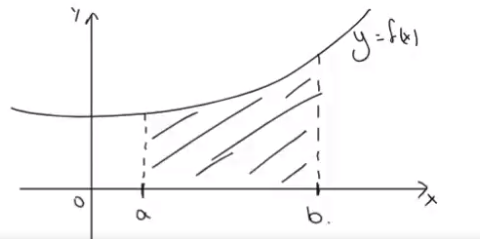
\includegraphics[scale=0.5]{app_of_calc_integ_1}
	\end{center}
	\begin{center}
		~\\
		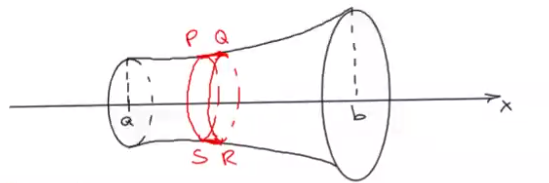
\includegraphics[scale=0.5]{app_of_calc_integ_2}
	\end{center}
\end{multicols}


Suppose that the solid formed is cut into sections as shown. Let $PQRS$ be a typical section. If the cuts are reasonably close to each other, $PQRS$ approximates a cylinder with height $\delta x$ and radius $y$ as shown below:
\begin{center}
	\qquad \qquad 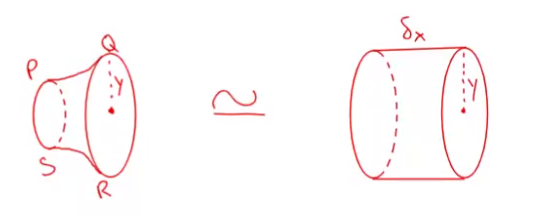
\includegraphics[scale=1]{app_of_calc_integ_3}
\end{center}
The volume, $\delta v$, of $PQRS$ is given by:
$$\delta V \simeq \pi y^2 \delta x$$
Thus, the volume $V$ of solid $PQRS$ is given by:
$$V\simeq \sum_{x=a}^{b} \pi y^2 \delta x$$
This summation approaches $V$ as $\delta x \to 0$
$$V = \lim\limits_{\delta x \to 0}   \sum_{x=a}^{b} \pi y^2 \delta x$$
$$\quad\boxed{V = \int_{a}^{b} \pi y^2 \, dx}$$
\hrulefill
\begin{example}
	Find the volume generated when the area  between $y=e^x$, the x-axis
\end{example}

\begin{alignat*}{2}
	&   & V & =\int_{0}^{1} \pi y \, dx \\
\end{alignat*}

\begin{example}
	Find the volume generated when the area defined by the inequalities $y\leq x^2$ and $y\geq x$ is rotated about the $x$-axis.
\end{example}
\begin{multicols}{2}
	\begin{tikzpicture}
		\begin{axis}[
			width=8cm,
			height=6cm,
			axis line style={-},
			xmin=0,
			xmax=2.5,
			ymin=0,
			ymax=2.5,
			xtick={}, % remove all ticks from x-axis
			ytick={}, % ditto for y-axis
			xlabel=$x$, 
			ylabel=$y$,
			axis lines=center, % default is to make a box around the axis
			samples=100]
			\addplot [name path=A,samples=501, domain=0:2, black] {sqrt(x)};
			\addplot [name path=B,samples=501, domain=0:2, green]  {x};
			\draw[pattern=north east lines,
			intersection segments={
				of=A and B,
				sequence={L2--R2[reverse]}
			}];
		\end{axis}
	\end{tikzpicture}
	\begin{center}
		
	\end{center}
	
\end{multicols}
\begin{alignat*}{2}
	&   & V_{e-c} & = V_e - V_c                                                      \\
	&   &         & = \pi \int_{0}^{1} \sqrt{x}^2 \, dx - \pi \int_{0}^{1} x^2 \, dx \\
\end{alignat*}
\begin{example}
	Find the volume generated when the area in the first quadrant bounded by the circle $x=4\cos\theta, y=4\sin\theta$ rotates completely about the $x$-axis.
\end{example}
\begin{example}
	
	Find the volume when the region defined by  $y\geq x^2+1,\quad x\geq0$ and $y\leq2$ is rotated about the $y$-axis.
\end{example}
\begin{tikzpicture}
	\begin{axis}[
		width=8cm,
		height=6cm,
		axis line style={-},
		xmin=0,
		xmax=2.5,
		ymin=0,
		ymax=2.5,
		xtick={}, % remove all ticks from x-axis
		ytick={}, % ditto for y-axis
		xlabel=$x$, 
		ylabel=$y$,
		axis lines=center, % default is to make a box around the axis
		samples=100]
		\path[name path=axis] (axis cs:0,0) -- (axis cs:0,2);
		\addplot [name path=A, domain=0:2, black] {2};	
		\addplot [name path=B, domain=0:2, black]  {x^2 + 1};
		\draw[pattern=north east lines,
		%TODO fix this
		intersection segments={
			of=B and A,
			of=axis and B,
			of=A and axis,
			sequence={L2--R	2[reverse]}
		}];
		%	\draw[pattern=north east lines,
		%	intersection segments={
		%		of=axis and B,
		%	}];
	\end{axis}
\end{tikzpicture}
\subsection{Length of an arc of a curve}
To find the length of an arc of a curve we use the method of summing small elements of one length.\\
Suppose that arc $PQ$, of length $\delta s$, is such an element. Then, the length $S$ of the curve $AB$ is given by:
\begin{multicols}{2}
	\begin{center}
		$\sum_{x=x_1}^{x_2} \delta S$
	\end{center}
	\begin{center}
		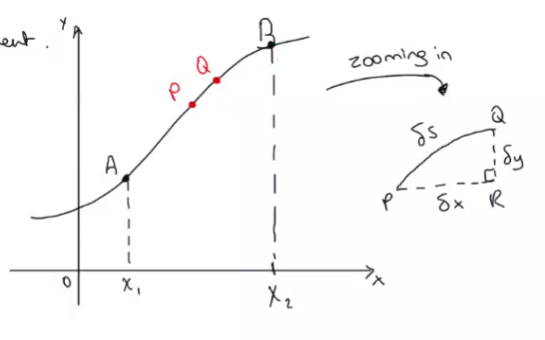
\includegraphics[width=0.7\linewidth]{app_of_integ_4}
	\end{center}
\end{multicols}


As $\delta s$ is very small, it can be approximated to the hypothenuse of the $\triangle PQR$. Thus:
\begin{alignat*}{2}
	&            & (\delta x)^2 + (\delta y)^2                    & \simeq (\delta s)^2                                                                 \\
	& \implies   & 1 + \left( \frac{\delta y}{\delta x}\right) ^2 & \simeq \left( \frac{\delta S}{\delta x}\right) ^2                                   \\
	& \implies   & \delta S                                       & \simeq \sqrt{1+\left( \frac{\delta y}{\delta x}\right)^2 } \delta x                 \\
	& \therefore & S                                              & \simeq \sum_{x=x_1}^{x_2} \sqrt{1 + \left(\frac{\delta y}{\delta x}\right)}\delta x 
\end{alignat*}
~\\
~\\
As $\delta x \leftarrow 0, (\frac{\delta y}{\delta x}) \leftarrow \frac{dy}{dx} \quad $and$ \quad s = \lim_{\delta x \to 0} \sum_{x=x_1}^{x_2} \sqrt{1+\left( \frac{\delta y}{\delta x}\right)^2}  \delta x$
~\\
~\\
~\\

\begin{center}
	\begin{tcolorbox}[center title,hbox,    
		lifted shadow={1mm}{-2mm}{3mm}{0.1mm}%
		{black!50!white}]
		\begin{varwidth}{\textwidth}
			\begin{center}
				$\therefore \quad S = \int_{x_1}^{x_2} \sqrt{1 + \left(\frac{dy}{dx}\right)^2}\, dx$
			\end{center}
		\end{varwidth}
	\end{tcolorbox} 
\end{center}


Knowing the Cartesian equation of the curve, the necessary integration can be carried out.\\

Let us now consider a curve $S$ parametrically in terms of $t$.

We can use again :
\begin{alignat*}{2}
	&          & (\delta s )^2                            & \simeq (\delta x)^2 + (\delta y)^2                                                                         \\
	& \implies & \left(\frac{\delta s}{\delta t}\right)^2 & \simeq \left(\frac{\delta x}{\delta t}\right)^2 + \left(\frac{\delta y}{\delta t}\right)^2                 \\
	& \implies & \delta s                                 & \simeq \sqrt{\left(\frac{\delta x}{\delta t}\right)^2 + \left(\frac{\delta y}{\delta t}\right)^2} \delta t 
\end{alignat*}

~\\
as $\delta t \to 0\quad ; \quad \frac{\delta x}{\delta t} \to \frac{dx}{dt} \quad \text{and} \quad \left(\frac{\delta y}{\delta t}\right) \to \frac{dy}{dt}$\\
~\\

$$\therefore S = \lim_{\delta t \to 0} \sum_{t=t_1}^{t_2} \sqrt{\left(\frac{\delta x}{\delta t}\right)^2 + \left(\frac{\delta y}{\delta t}\right)^2} \delta t$$

\begin{center}
	\begin{tcolorbox}[center title,hbox,    %%<<---- here
		lifted shadow={1mm}{-2mm}{3mm}{0.1mm}%
		{black!50!white}]
		\begin{varwidth}{\textwidth}
			\begin{center}
				$S = \int_{t_1}^{t_2} \sqrt{\left(\frac{dx}{dt}\right)^2 + \left(\frac{dy}{dt}\right)^2}\, dt$
			\end{center}
		\end{varwidth}
	\end{tcolorbox} 
\end{center}
\section{Rates of change}
The notation $\dfrac{dy}{dx}$ denotes the rate of change of $y$ w.r.t.x. Suppose that $x$ and $y$ are quantities a such as length and volume respectively. Then $\dfrac{dy}{dx}$ denotes the rate of change of volume w.r.t some length. In this section we use differentiation to deal with practical problems involving rates of change. 

\begin{example}
	A spherical balloon is blown up so that its volume increases at a constant rate of $2\text{cm}^3/s$. Find the rate of increase of the radius when the volume of the balloon is $50\text{cm}^3$
\end{example}

\begin{multicols}{2}
	$\od{V}{t} = 2$
	
\end{multicols}
\begin{example}
	A container with water is in the form of an inverted hollow cone with a iaerrentical angle of $30\degree$. Water drips out from the vertex at the rate $3\text{cm}^2/s$. Find the rate at which the surface area in contact with the water is changing when there are $8\pi\text{cm}^3$ of water remaining in the cone.
	
	\begin{figure}
		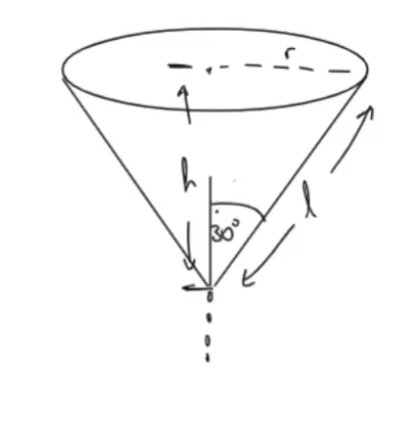
\includegraphics[scale=0.5]{app_of_calc_der_1}
	\end{figure}
	\begin{multicols}{2}
		\begin{align*}
			\od{V}{t} & = -3                            \\
			V         & = \frac{1}{3} \pi r^2 h         \\
			V         & = \frac{1}{3} \pi r^2 \sqrt{3}r \\
			V         & = \frac{\sqrt{3}}{3}\pi r^3     \\
			\od{V}{t} & = \sqrt{3}\pi  r^2              
		\end{align*}
		\begin{align*}
			\text{Required derivative: } \od{A}{t} &          \\
			A                                      & = \pi rl 
		\end{align*}
		
	\end{multicols}
\end{example}
\end{document}
	